% Page budget: 1.5--2 pages within Section 7.
\subsection{Cross-audit financial resource optimization}
\label{sec:financial-compression-audit}

The two licensed-data exercises are complementary retrospective protocols
with different decision timing and held-out outcome units.  The terminal
financial audit makes one fixed holdout evaluation after development and
validation; the annual walk-forward financial audit makes five target-year
decisions using trailing information through the preceding year.  Neither
protocol supersedes the other, and their held-out quality levels are not
pooled.  Both compare a current stepwise safe library with HiGHS-reported
minimum-cardinality and minimum-validation-resource candidates.  The terminal
audit starts from $80$ strategies, $38$ modules, and validation-computation
burden $1558$; the annual walk-forward audit starts from $202$ strategies,
$113$ modules, and burden $3508$.  Validation frontiers and structural
closure are available at compression time.  Held-out descendant quality is
read only after each decision and is used solely as an ex post opportunity
diagnostic; neither pruning rule tests candidate-set equality.  Appendix~E
gives the complete information set and solver
qualifications; Online Supplement~S6 gives the formulas and secondary tests.

\begin{table}[htbp]
\centering
\scriptsize
\setlength{\tabcolsep}{3.2pt}
% Generated by julia/scripts/generate_main_text_tables.jl.
% Exact source: experiments/results/summaries/financial_resource_optimization_solutions.csv.
\begin{tabular}{@{}lccccc@{}}
\toprule
Audit & Source & Stepwise safe & HiGHS min-card. & HiGHS min-\(W_v\) & Frontier-only \\
 & \((|L|,W_v)\) & \((|L|,W_v)\) & \(|L|\) & \((|L|,W_v)\) & \((|L|,W_v)\) \\
\midrule
Terminal & \((80,1558)\) & \((25,450)\) & \(25\) & \((25,338)\) & \((3,64)\) \\
Annual & \((202,3508)\) & \((100,1566)\) & \(100\) & \((100,1170)\) & \((5,44)\) \\
\bottomrule
\end{tabular}

\caption{Cross-audit financial resource optimization.  \(|L|\) is a strategy count and
\(W_v\) is measured in prespecified validation-computation units.  ``HiGHS''
means the mixed-integer solver reported \texttt{OPTIMAL}; it does not mean
exact global optimality was established by enumeration.  Selected libraries,
burdens, frontiers, and closures are rechecked exactly.}
\label{tab:financial-resource-compression}
\end{table}

HiGHS reports that the stepwise endpoints already match its minimum-cardinality
candidates: both retain $25$ and $100$ strategies, respectively, although
distinct HiGHS-reported minimizing libraries can use different identities.
The HiGHS-reported minimum-weight safe candidates keep those cardinalities but
lower burden from
$450$ to $338$ and from $1566$ to $1170$.  Relative to the source, the savings
are $1220$ units
$(78.31\%)$ and $2338$ units $(66.65\%)$; relative to the current
stepwise endpoints, the HiGHS-reported weight candidates save a further $24.89\%$
and $25.29\%$.  Every safe library in the comparison preserves the complete
frontier and all $38$ or $113$ source modules, and its ex post
enabled-descendant opportunity quality is unchanged.

Frontier-only compression retains just $3$ and $5$ strategies and only
$12/38$ and $14/113$ modules.  Its ex post opportunity diagnostic falls by
$0.0016$ and $0.1020$ in the audits' distinct units.  The resulting
safety--compression trade-off is stark: minimum-cardinality safe compression
removes $68.75\%$ and $50.50\%$ of strategies while preserving closure;
frontier-only compression removes $96.25\%$ and $97.52\%$, but breaks
closure and loses the best held-out enabled opportunity in both audits.

\begin{figure}[htbp]
  \centering
  % Generated by julia/scripts/generate_manuscript_numerical_artifacts.jl.
% Sources: registered financial mechanism, decomposition, grammar, candidate-audit,
% and annual episode-ranking CSVs. The locked scoring engines are not rerun here.
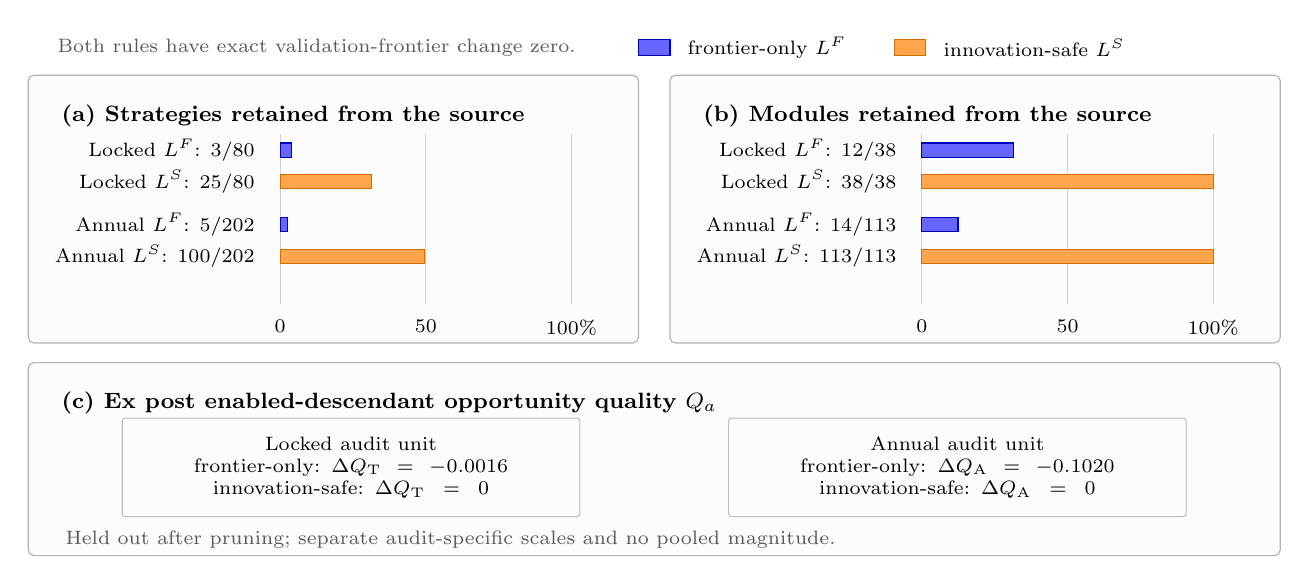
\begin{tikzpicture}[x=1cm,y=1cm,font=\scriptsize]
  \tikzset{
    panel/.style={draw=black!30,rounded corners=2pt,fill=black!1},
    frontier/.style={draw=blue!72!black,fill=blue!60},
    safe/.style={draw=orange!85!black,fill=orange!70},
    title/.style={font=\bfseries\footnotesize,anchor=north west},
    note/.style={font=\scriptsize,anchor=west,text=black!65},
    card/.style={draw=black!25,rounded corners=1pt,align=center,inner sep=3pt}
  }

  % Shared legend and exact zero-frontier-change qualification.
  \draw[frontier] (7.75,6.35) rectangle (8.15,6.55);
  \node[anchor=west] at (8.25,6.45) {frontier-only \(L^F\)};
  \draw[safe] (11.00,6.35) rectangle (11.40,6.55);
  \node[anchor=west] at (11.50,6.45) {innovation-safe \(L^S\)};
  \node[anchor=west,text=black!65] at (0.25,6.45)
    {Both rules have exact validation-frontier change zero.};

  % (a) Fraction of source strategies retained.
  \draw[panel] (0,2.70) rectangle (7.75,6.10);
  \node[title] at (0.30,5.85) {(a) Strategies retained from the source};
  \foreach \x/\label in {3.2/0,5.05/50,6.9/100\%} {
    \draw[black!18] (\x,3.20) -- (\x,5.35);
    \node[anchor=north] at (\x,3.12) {\label};
  }
  \node[anchor=east] at (3.00,5.15) {Locked \(L^F\): 3/80};
  \draw[frontier] (3.2,5.06) rectangle (3.33875,5.24);
  \node[anchor=east] at (3.00,4.75) {Locked \(L^S\): 25/80};
  \draw[safe] (3.2,4.66) rectangle (4.35625,4.84);
  \node[anchor=east] at (3.00,4.20) {Annual \(L^F\): 5/202};
  \draw[frontier] (3.2,4.11) rectangle (3.291584,4.29);
  \node[anchor=east] at (3.00,3.80) {Annual \(L^S\): 100/202};
  \draw[safe] (3.2,3.71) rectangle (5.031683,3.89);

  % (b) Fraction of source modules retained.
  \draw[panel] (8.15,2.70) rectangle (15.90,6.10);
  \node[title] at (8.45,5.85) {(b) Modules retained from the source};
  \foreach \x/\label in {11.35/0,13.2/50,15.05/100\%} {
    \draw[black!18] (\x,3.20) -- (\x,5.35);
    \node[anchor=north] at (\x,3.12) {\label};
  }
  \node[anchor=east] at (11.15,5.15) {Locked \(L^F\): 12/38};
  \draw[frontier] (11.35,5.06) rectangle (12.518421,5.24);
  \node[anchor=east] at (11.15,4.75) {Locked \(L^S\): 38/38};
  \draw[safe] (11.35,4.66) rectangle (15.05,4.84);
  \node[anchor=east] at (11.15,4.20) {Annual \(L^F\): 14/113};
  \draw[frontier] (11.35,4.11) rectangle (11.808407,4.29);
  \node[anchor=east] at (11.15,3.80) {Annual \(L^S\): 113/113};
  \draw[safe] (11.35,3.71) rectangle (15.05,3.89);

  % (c) Ex post enabled-descendant quality; audit units are not pooled.
  \draw[panel] (0,0) rectangle (15.90,2.45);
  \node[title] at (0.30,2.20) {(c) Ex post enabled-descendant opportunity quality \(Q_a\)};
  \node[card,text width=5.60cm,minimum height=1.25cm] at (4.10,1.12)
    {Locked audit unit\\frontier-only: \(\Delta Q_{\mathrm T}=-0.0016\)\\
     innovation-safe: \(\Delta Q_{\mathrm T}=0\)};
  \node[card,text width=5.60cm,minimum height=1.25cm] at (11.80,1.12)
    {Annual audit unit\\frontier-only: \(\Delta Q_{\mathrm A}=-0.1020\)\\
     innovation-safe: \(\Delta Q_{\mathrm A}=0\)};
  \node[note] at (0.35,0.20) {Held out after pruning; separate audit-specific scales and no pooled magnitude.};
\end{tikzpicture}

  \caption{Financial safety--compression trade-off for the current stepwise
  endpoints.  Panels (a)--(b) report exact retained fractions of each fixed
  source library and module closure.  Panel (c) reports
  \(\Delta Q_a=Q_a(L')-Q_a(L)\), the held-out change in the best enabled
  descendant's audit-specific opportunity quality; the two audit units are
  not pooled.  Both rules preserve the validation frontier, but only the safe
  rule preserves closure and \(Q_a\).  The displayed \(Q_a\) values are
  rendered audit decimals and are not pruning inputs.  \Cref{tab:financial-resource-compression}
  adds the HiGHS-reported minimum-cardinality and minimum-weight comparisons.}
  \label{fig:financial-safe-compression}
\end{figure}

\clearpage
The secondary coverage-ranking stress test is adverse in the terminal audit
and mixed in the five annual targets.
Coverage scores are post-compression ranking inputs, never pruning inputs.
The terminal coverage-ranked set has
locked utility $-0.1560$, versus $-0.0685$ for the strongest comparator,
with Spearman association $-0.0982$.  Annual marginal coverage averages
$0.0704$, versus $0.0119$, but is positive in only three of five targets;
mean Spearman association is $0.1279$ and greedy-oracle regret is $0.315$.
These retrospective quantities neither identify expected return nor establish
market alpha.  The secondary figure and full estimates are online.
